% !TeX program = xelatex
\documentclass{scrartcl}

% This commad is defined in the makefile to generate the different
% language versions. If one compiles it directly this fallback is active.
\providecommand{\SelectedLanguage}{english}

% This commad is defined in the makefile to select a random color scheme.
% If one compiles it directly this fallback is active.
\providecommand{\SelectedColorSchemeNumber}{5}% = random

\RequirePackage{polyglossia}
   \setmainlanguage{\SelectedLanguage}

\usepackage{microtype}

\usepackage[
%   color-mode = gray,
   color-scheme-number = \SelectedColorSchemeNumber,
%   load-fonts = false,
]{citobiw}

\usepackage[
   language = \SelectedLanguage,
   show-frame,
   year-format = YY,
]{cvtobiw}

\usepackage{hyperref}
   \urlstyle{same}

\newcommand{\softwareskills}{%
   Adobe CC (InDesign, InCopy,\linebreak Illustrator, Photoshop),
   Word, Excel, Powerpoint,
   Pages, Numbers, \mbox{Keynote},
   \TeX/,
   Terminal/Konsole,\linebreak
   Sibelius, Finale
}
\newcommand{\codingskills}{%
   \skill{\LaTeXe/}{90}\\
   \skill{\LaTeXiii/}{85}\\
   \skill{\TikZ/}{90}\\
   \skill{HTML\,5}{80}\\
   \skill{CSS\,3}{80}\\
   \skill{PHP}{70}\\
   \skill{Java/JavaScript}{40}
}
\newcommand{\osskills}{%
   \skill{Mac OS X}{100}\\
   \skill{Linux (Ubuntu)}{65}\\
   \skill{Windows}{45}
}

\begin{document}

\begin{languagecontent}{german}
   \setvar{main}{%
      \textcp{\textbf{Hallo.}}
      
      Darf ich mich Ihnen vorstellen? Ich bin Tobias Weh, Lehrer und freier Grafiker
      aus Osnabrück. Neben der Physik und der Musik schlägt mein Herz vor allem für
      Buchstaben, Typografie und natürlich gute Gestaltung. \emph{Design} bedeutet
      für mich in erster Linie das Lösen von einem konkreten Problem, um damit Ihnen
      oder Ihren Kunden das Leben in gewisser Weise zu erleichtern – zum Beispiel
      durch eine schnell und einfach zu erfassende Darstellung von Informationen.
      Erst wenn so eine Lösung gefunden ist, kann man sie mit gestalterischen Mitteln
      und sauberem Handwerk in eine ästhetische Form bringen und damit eine
      nachhaltige und gute Gestaltung erreichen.
      
      Ich stehe Ihnen gerne zur Verfügung, um mit Ihnen gemeinsam ein Erscheinungsbild
      (\emph{Corporate Design}) zu entwickeln, für Ihre Texte oder Noten ein
      angemessenes Layout zu finden und sie zu setzen, für Ihr Buch anschauliche
      Abbildungen anzufertigen oder um Sie in allen Fragen rund um \TeX/ zu beraten.
      
      Herzliche Grüße\\
      Tobias Weh
   }

   \setvar{contact}{%
      T\kern-1ptobias W\kern-0.4pteh\\
      Spindelstraße 25\\
      40980 Osnabrück
      
      05\kern0.2pt4\kern-0.2pt1\,·\,40\kern-0.1pt757837\\
      0\kern-0.2pt160\,·\,5063337
      
      \href{mailto:mail@tobiw.de}{mail\raisebox{0.1ex}{@}tobiw\kern-0.75pt.de}\\
      \href{http://tobiw.de}{tobiw\kern-0.75pt.de}
   }

   \setvar{skills}{
      \minisec{Sprachen}
      \skill{Deutsch}{100}\\
      \skill{Englisch}{75}
      
      \minisec{Programme}
      \softwareskills
      
      \minisec{Programmiersprachen}
      \codingskills
      
      \minisec{Systeme}
      \osskills
   }

   \setvar{timeline-entries}{
      \timelineentry{1988}{geboren in Stadthagen bei Hannover}{}[28]
      \timelineentry{2007}{Abitur am Fachgymnasium Technik, Stadthagen}
         {Leistungskurse: Deutsch und\linebreak Elektrotechnik}
      \timelineentry{2007-2008}[14]{Freiwilliges Soziales Jahr Kultur}
         {Im Rahmen meines FSJ beim Landesmusikrat Niedersachsen e.\,V.
         habe ich diverse Projekte wie \emph{Jugend musiziert}
         mitorganisiert und durchgeführt.}[14]
      \timelineentry{2008-2014}{Studium an der Uni Osnabrück}
         {Lehramt für Gymnasium\\(Physik und Musik)}
      \timelineentry{2011-2014}[1]{\TeX/-Kurse}
         {Im Fachbereich Physik der Uni Osnabrück habe ich \TeX/-Kurse gegeben.}
      \timelineentry{2012}[2]{Bachelorarbeit}
         {„Entwicklung des Java-Programms FIELDS zur zweidimensionalen\linebreak Darstellung
         von Feldern mithilfe des PhidgetInterfaceKit 2/2/2“}[11]
      \timelineentry{2014}[2]{Masterarbeit}
         {„Anschauliche Erklärung der trans\-mittierten und reflektierten Schallwellen
         am Ende einer offenen Röhre“}[11]
      \timelineentry{2011-today}[15]{selbstständige T\kern0.1ptätigkeit}
         {als Grafiker, Setzer, \TeX/-Berater}
      \timelineentry{2012-2014}[16]{wissenschaftliche Hilfskraft}
         {Betreuung der Internetseite (Typo3)\linebreak des Instituts für Musik der\linebreak Uni Osnabrück}
      \timelineentry{2013-mid2013}[17]{wissenschaftliche Hilfskraft}
         {Tutor in der Physikdidaktik an der Uni Osnabrück}[10]
      \timelineentry{2014-today}[17]{Studium an der FH Bielefeld}
         {Bachelor Gestaltung\\(Grafik und Kommunikationsdesign)}
   }

   \setvar{code}{
      Erstellt mit \TeX/ – Code auf \href{https://github.com/tweh/cv}{github.com/tweh/cv}.
   }
\end{languagecontent}

\begin{languagecontent}{english}

   \setvar{contact}{%
      T\kern-1ptobias W\kern-0.4pteh\\
      Spindelstraße 25\\
      40980 Osnabrück\\
      Germany\\[0.5\baselineskip]
      %
      +49\,5\kern0.2pt4\kern-0.2pt1\,·\,40\kern-0.1pt757837\\
      +49\,160\,·\,5063337\\[0.5\baselineskip]
      %
      \href{mailto:mail@tobiw.de}{mail\raisebox{0.1ex}{@}tobiw\kern-0.75pt.de}\\
      \href{http://tobiw.de}{tobiw\kern-0.75pt.de/\kern-0.5pten}
   }

   \setvar{skills}{
      \minisec{Languages}
      \skill{German}{100}\\
      \skill{English}{80}
      
      \minisec{Software}
      \softwareskills
      
      \minisec{Programming Languages}
      \codingskills
      
      \minisec{Operating Systems}
      \osskills
   }

   \setvar{code}{
      Made with \TeX/ – Code at \href{https://github.com/tweh/cv}{github.com/tweh/cv}
   }
\end{languagecontent}

\setvar{image}{%
   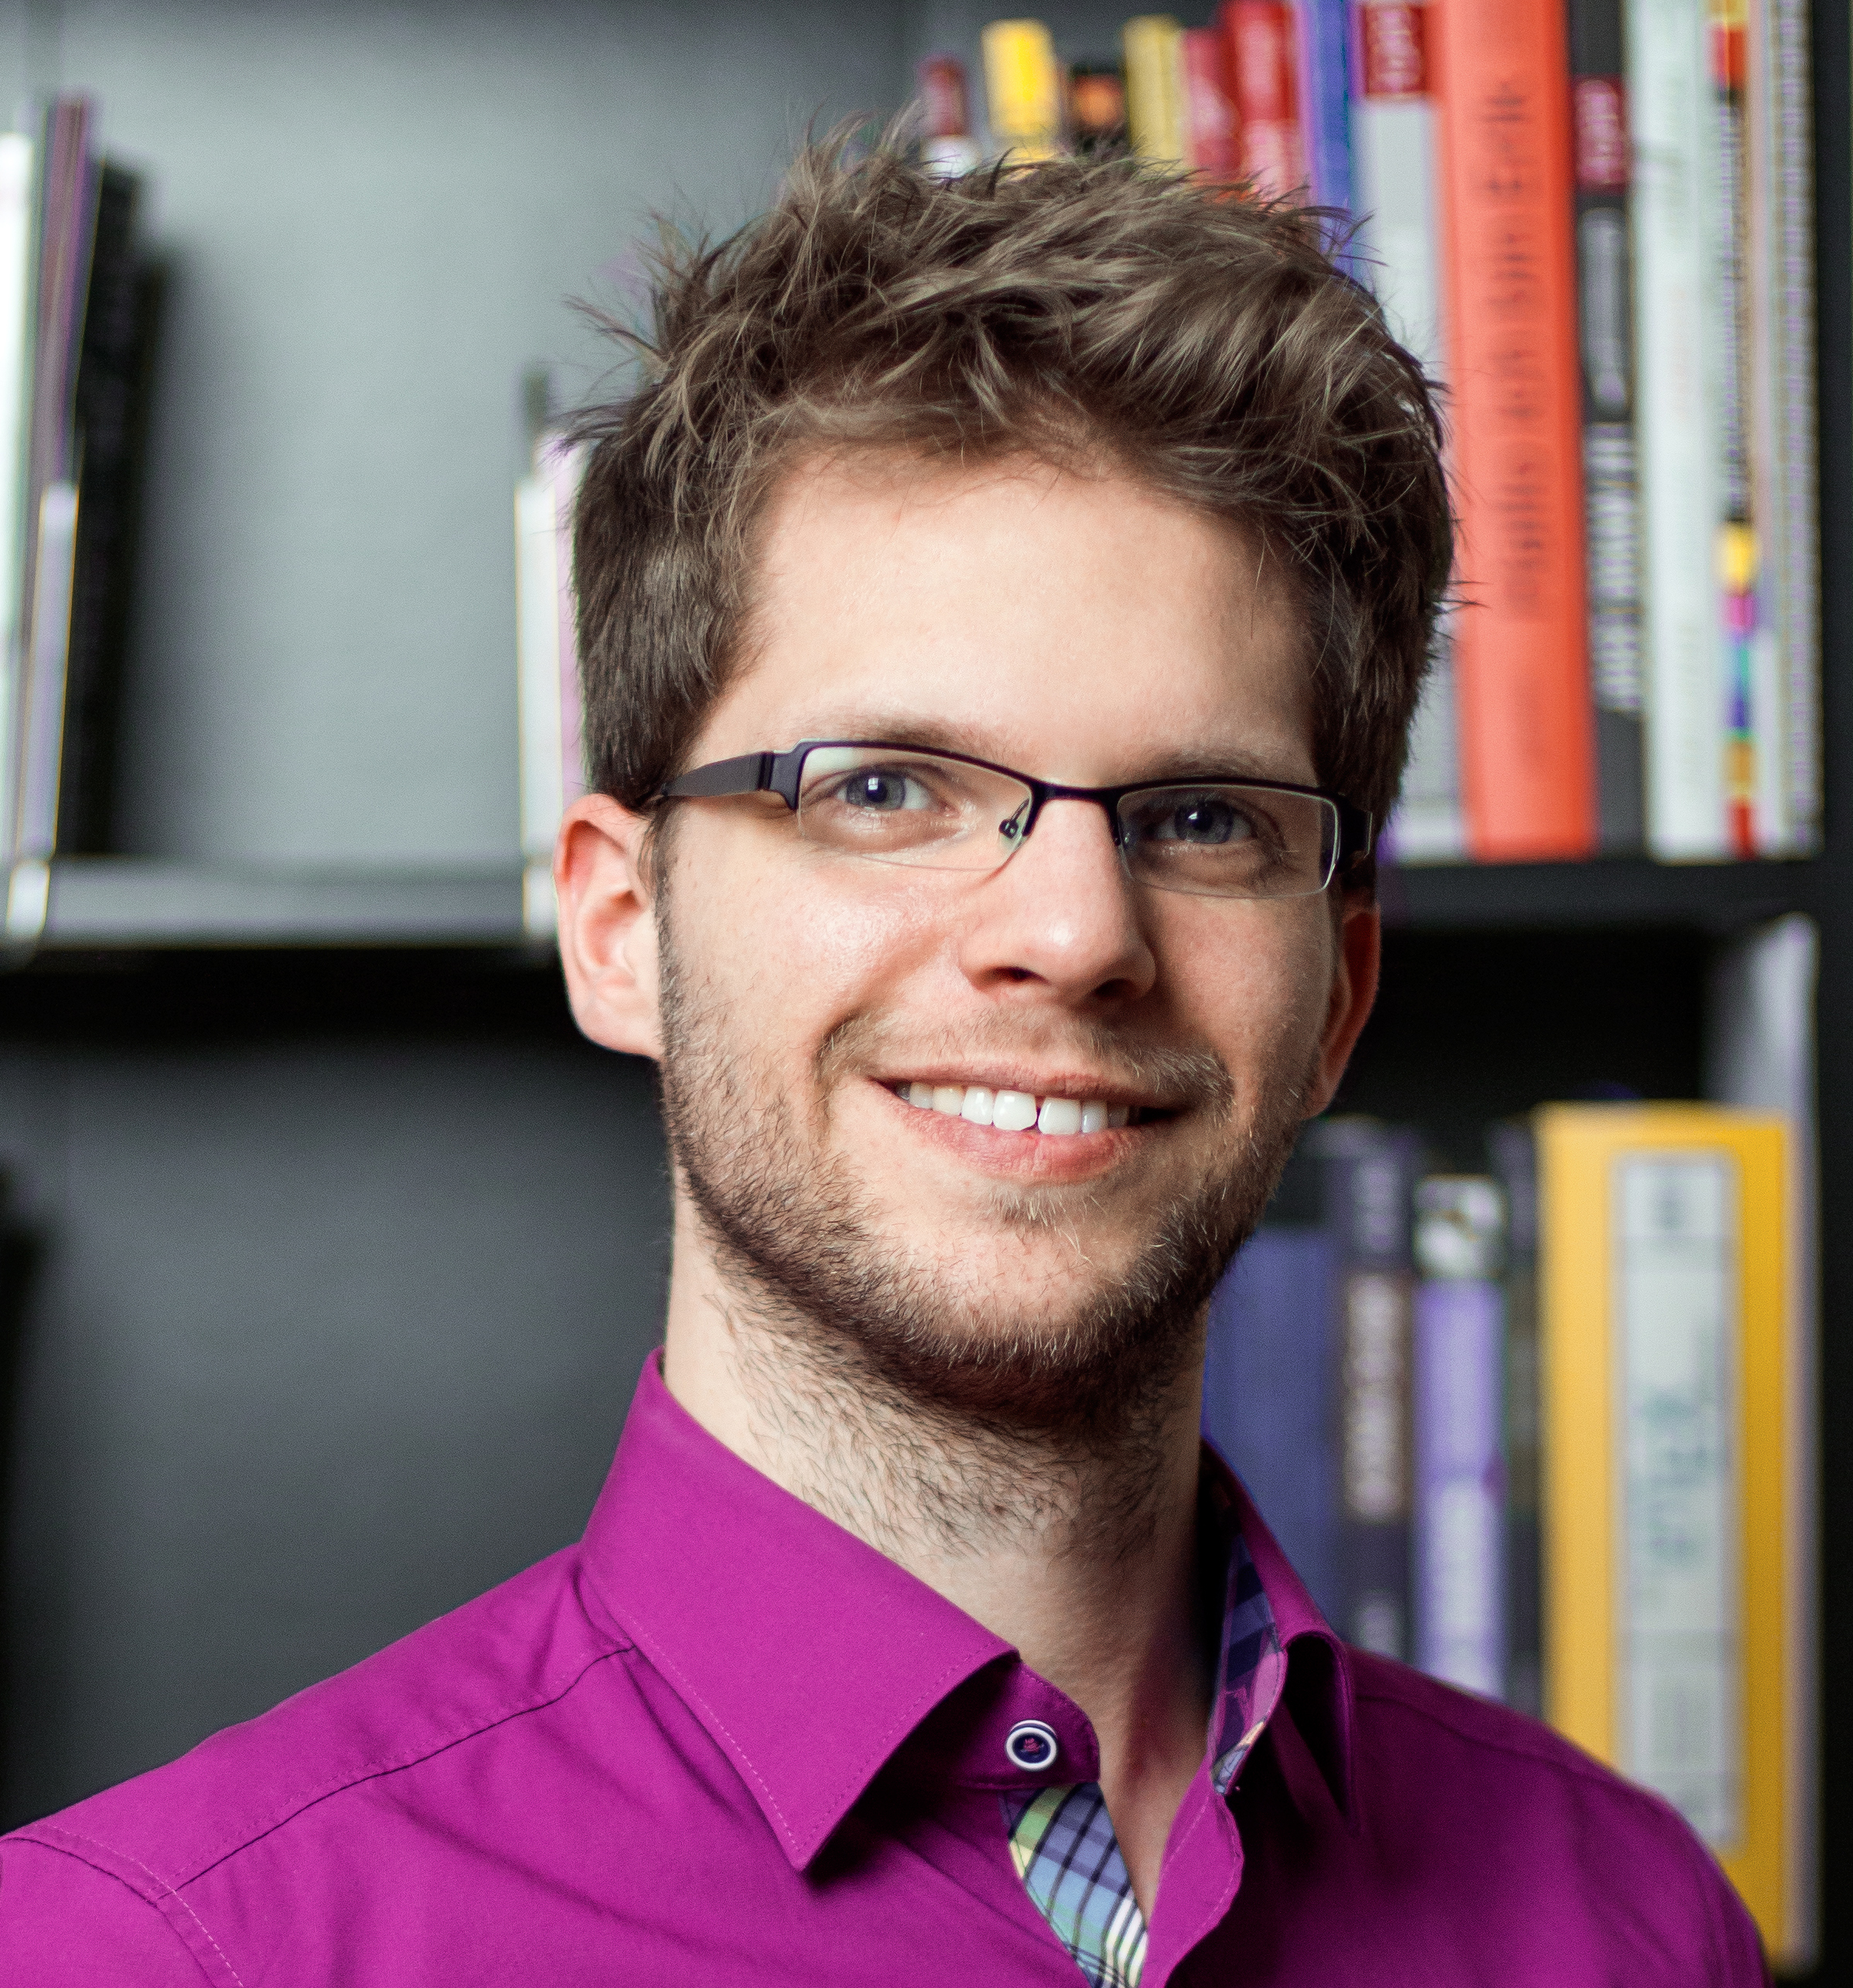
\includegraphics[width=\usedim{right-col-width}]{img/tobiw}
}

\setvar{logo}{%
   \TobiWLogo[height=4ex]
}

\setvar{timeline-birth}{1988}
\setvar{timeline-start}{2007}
\setvar{timeline-end}{2015}

%\MakeCV

\newproject{one}
\newproject{two}
\newproject{three}
\newproject{four}

\newproject{de}
\newproject{en}
\newproject{all1}
\newproject{all2}

\setprojectvar{all1}{title}{Allgemeines Projekt 1}
\setprojectvar{all1}{content}{Beschreibung für Allgemeines Projekt 1}
\setprojectvar{all2}{title}{Allgemeines Projekt 2}
\setprojectvar{all2}{content}{Beschreibung für Allgemeines Projekt 2}

\begin{languagecontent}{german}

   \setprojectvar{de}{title}{Deutsches Projekt}
   \setprojectvar{de}{content}{Beschreibung für Deutsches Projekt}

   \setprojectvar{one}{title}{Projekt Eins}
   \setprojectvar{one}{content}{Inhalt 1}
   
   \setprojectvar{two}{title}{Projekt Zwei}
   \setprojectvar{two}{content}{Inhalt 2}
%   
%   \setprojectvar{three}{title}{Projekt Drei}
%   \setprojectvar{three}{content}{Inhalt 3}
%   
%   \setprojectvar{four}{title}{Projekt Vier}
%   \setprojectvar{four}{content}{Inhalt 4}

\end{languagecontent}
\begin{languagecontent}{english}

   \setprojectvar{en}{title}{Englisches Projekt}
   \setprojectvar{en}{content}{Beschreibung für Englisches Projekt}

%   \setprojectvar{one}{title}{Project One}
%   \setprojectvar{one}{content}{Content 1}
   
%   \setprojectvar{two}{title}{Project Two}
%   \setprojectvar{two}{content}{Content 2}
%   
   \setprojectvar{three}{title}{Project Three}
   \setprojectvar{three}{content}{Content 3}
%   
%   \setprojectvar{four}{title}{Project Four}
%   \setprojectvar{four}{content}{Content 4}

\end{languagecontent}

\MakePortfolio[one,en,three]

\end{document}